\makeatletter \@ifundefined{rootpath}{\input{../../setup/preamble.tex}}\makeatother
\worksheetstart{Evaluation}{1}{Marts 2, 2015}{Andreas}{../../}
This chapter evaluates \stmname, its associated \ac{STM} library and locking in C\# according to the characteristics defined in \cite[p. 15-21]{dpt907e14trending}. The evaluation will facilitate a conclusion on whether or not language integrated \ac{STM} is a valid alternative to locking as well as discerning whether language integration of \ac{STM} provides any advantages over library based \ac{STM} in terms of usability.
\label{chap:evaluation}
\section{Selected Problems}
As described in \bsref{sec:problem_statement} the evaluation will be conducted by comparing the characteristics of each approach based on a number of concurrent implementations. For this purpose three concurrency problems have been selected:
\begin{enumerate}
\item The dining philosophers problem\cite[p. 673]{hoare1978communicating}
\item The santa claus problem\cite{trono1994new}
\item A concurrent hashmap implementation\cite[p. 253]{cormen2009introduction}
\end{enumerate}
The dining philosophers problem represents a well known concurrency problem which highlights some of the pitfalls associated with conditional synchronization of threads. The Santa Claus problem encompasses a high degree of modeling and requires complex synchronization. Employing this problem helps investigate whether \ac{STM} provides any advantages over locking in such scenarios. Finally a concurrent hashmap implementation represents a real world problem, which benefits from fine grained synchronization and is used in many concurrent implementations. Together these problems provide a varied perspective by exerting different aspects of each approach e.g. waiting on one of multiple conditions and fine grained synchronization.

\section{Evaluation Approach}
For each of the selected problems an implementation will be created using, locking, library based \ac{STM} and language based \ac{STM}. Based on these implementations each concurrency approach will be evaluated according to the characteristic defined in our previous work 
\cite[p. 15-21]{dpt907e14trending}. While each of these characteristics range from one extreme to another, e.g. high or low readability, a concurrency approach may not reside at one of these extremes, but more likely somewhere in between. Therefore, as part of the evaluation, each concurrency approach will be given a placement on the spectrum of each characteristic, based on findings in the evaluation. In order to visualize this placement a scale similar to one presented in \bsref{fig:evel_example} is employed. Here \bscode{X} and \bscode{Y} represent the two extremes of the spectrum while the indicators represent the placement of each of the concurrency approaches on the spectrum. As an example \bscode{X} and \bscode{Y} could be low and high writability, \bsref{fig:evel_example} then shows that each of the concurrency approaches resides more towards the high writability end of the spectrum.
\begin{figure}[ht!]
\centering
\includegraphics[scale=0.5]{\rootpath/worksheets/evaluation/figures/eval_example}
\caption{Example of characteristic evaluation scale}\label{fig:evel_example}
\end{figure}
Giving each concurrency approach a visual placement allows for improved communication of the findings along with the ability to easily compare the placement of each concurrency approach.

\section{Implementations}
To ensure common ground between all implementations of a particular problem, a set of requirements detailing common factors which must be true for all implementations of a particular problem has been created.

The dining philosophers implementations must:
\begin{itemize}
	\item Encompass two 100 milliseconds thread sleeps. One to exemplify the act of eating as well as one upon completing an attempt to eat exemplifying sleeping a period before attempting to eat again.
\end{itemize}

The santa claus problem implementations must:
\begin{itemize}
	\item Follow the requirements defined in \cite{trono1994new}
	\item Utilize advantageous features of the concurrency approach.
\end{itemize}

The concurrent hashmap implementations must:
\begin{itemize}
	\item Encompass fined grained synchronization, allowing multiple threads to operate on the hashmap simultaneously.
\end{itemize}
The implementations in their full length can be found in the appendix.\toby{indsæt et reference når de indsætts}

\section{Evaluation of Characteristics}
All of the selected concurrency approaches relies on starting threads in order to introduce concurrency as well as manually specifying critical regions using ether locks or the \bscode{atomic} block. 
\toby[i]{Noget intro tekst her, ellers kan sektionen vel ligeså godt slettes og undersektioner gøres til sektioner?}
\subsection{Implicit or Explicit Concurrency}
The two \ac{STM} based approaches have implicit elements\toby{Ved ikke om man kan sige det med elements? Måske brug features istedet, eller formuler det til at det det er mere implicit eller mere mod den implicitte ende? (elements udtrykket er brugt i næste subsektion også)} as \ac{STM} allows them to hide the details synchronization. Locking in C\# on the other hand requires explicit stating how synchronization is to be achieved. As such we say that locking in C\# resides close to the explicit concurrency extreme\toby{har vi en grund til at den ikke ligger på explicit? - vil Lone nok spørge} while \stmnamesp and the \ac{STM} library resides slightly more towards the implicit concurrency end of the spectrum. The placement of the three concurrency approaches on the implicit - explicit concurrency spectrum is depicted in \bsref{fig:char_implicit_explicit}.

\begin{figure}[htbp]
\centering
 \includegraphics[width=0.9\textwidth]{\rootpath/worksheets/evaluation/figures/char_implicit_explicit} 
 \caption{Concurrency approaches on the implicit - explicit concurrency spectrum}
\label{fig:char_implicit_explicit}
\end{figure}

\subsection{Fault Restrictive or Expressive}
Locking presents the programmer with a set of tools aimed at solving concurrency problems but does little to guarantee their correct usage. Locking in C\# provides the \bscode{lock} statement\cite[p. 102]{csharp2013specificaiton}, which defines a scope within which a given lock is held. The \bscode{lock} statement handles lock acquisition and release which removes the threat of programmers unintentionally missing to release an acquired lock. The lock statement is however only applicable in some scenarios and does, for example, not support timeouts on lock acquisition. As such, we say that locking in C\# resides at the expressive end of the spectrum.

The \ac{STM} based approaches delegate the details of how synchronization is achieved to the underling \ac{STM} system, allowing \ac{STM} based concurrency to avoid some of the errors associated with locking, such as deadlocks. The \ac{STM} based approaches however still rely on shared memory for communication and require programmers to define transaction scopes and introduce concurrency by starting threads. As such the \ac{STM} based approaches reside towards the expressive end of the spectrum but contain elements of fault restrictions pulling it more towards the fault restrictive extreme than locking. The placement of the three concurrency approaches on the fault restrictive - expressive spectrum is depicted in  \bsref{fig:char_fault_expressive}. 
\begin{figure}[htbp]
\centering
 \includegraphics[width=0.9\textwidth]{\rootpath/worksheets/evaluation/figures/char_fault_expressive} 
 \caption{Concurrency approaches on the fault restrictive - expressive spectrum}
\label{fig:char_fault_expressive}
\end{figure}

\subsection{Pessimistic or Optimistic}
Locking assumes that errors are common and therefore allows only a single thread to access a given critical region at a time, by enforcing mutual exclusion. As such locking is an inherently pessimistic concurrency approach. \ac{STM} on the other hand allows multiple threads to proceed simultaneously, correcting any errors that may occur by aborting and re-executing transactions. Hence \ac{STM} takes an optimistic approach to concurrency.
Therefore we say that \stmnamesp and the \ac{STM} library resides at the optimistic extreme of the pessimistic - optimistic spectrum while locking resides at the pessimistic extreme. The placement of the three concurrency approaches on the fault restrictive - expressive spectrum is depicted in \bsref{fig:char_pes_opti}. 
\begin{figure}[htbp]
\centering
 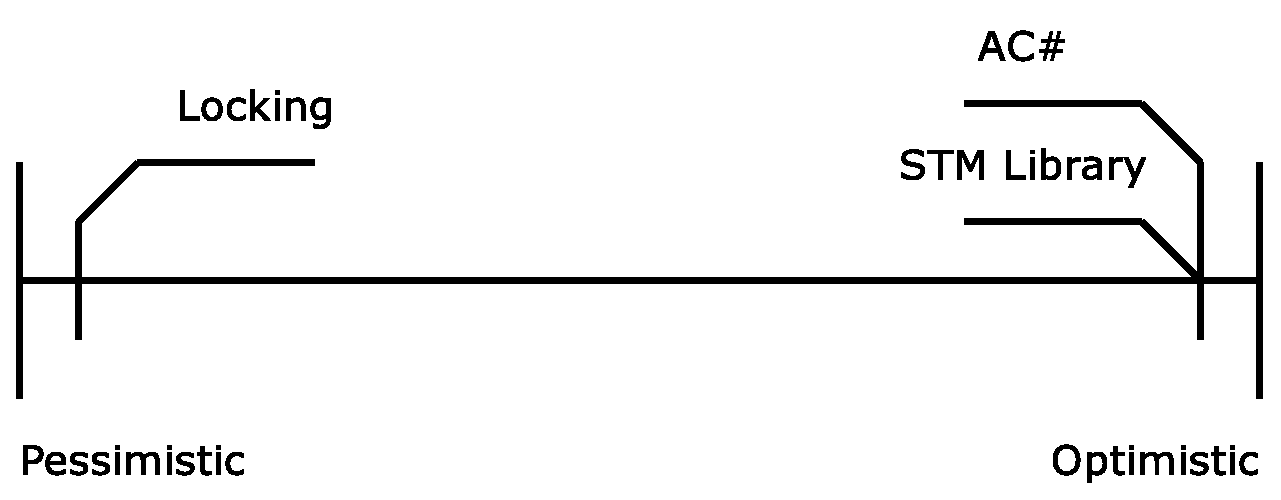
\includegraphics[width=0.9\textwidth]{\rootpath/worksheets/evaluation/figures/char_pessimistic_optemistic} 
 \caption{Concurrency approaches on the pessimistic - optimistic spectrum}
\label{fig:char_pes_opti}
\end{figure}

\subsection{Readability \& Writability}\label{subsec:tl_charac_read_and_write}
The evaluation of readability and writability are based on a number of shared criteria: Simplicity, Orthogonality, Data Types, and Syntax Design. The last two comes in addition to the criteria used in the evaluation model defined in our prior work\cite[p. 16-21]{dpt907e14trending}. The reason being, that it is now a concurrency approach in a language, and not the isolated concurrency model. In addition to the shared criteria, writability is based on the level of abstraction and expressivity.
%that of simplicity and orthogonality as well as a number of other considerations. Simplicity and orthogonality is described in the following sections followed by a final evaluation of readability.
\subsubsection{Low or High Simplicity}\label{subsec:simplicity}
Locking in itself is only a single construct in C\#. The construct is simple due to its low level of functionality, and requires the programmer to explicitly make usage of the construct to ensure correct synchronization. Both library based \ac{STM} and \stmname takes a more declarative approach than locking when specifying what needs to be synchronized, thus it is simpler as the programmer do not have to worry about the lower level details.\andreas{Skal vi have usability study ind igen?} In the case where conditional synchronization is needed, both forms of \ac{STM} can leverage the \bscode{retry} functionality and make the program wait until changes happens to the variables of the transaction.\andreas{Retry i santa example} In C\# a \bscode{Monitor} enables waiting until a lock has been freed, but contrary to \bscode{retry} this is not on a declarative level.

Library based \ac{STM} uses existing constructs, but does not support the implicit dependency between the static calls, e.g. \bscode{retry} only takes effect inside an \bscode{atomic} call. Additionally, the \ac{STM} types provided must be used to be tracked in transaction. These types causes a type mismatch when used together with standard types, thus making the library more complex to use. This issue is eased by providing implicit type conversion on the \ac{STM} types, but the implicit conversion is not possible in all cases. In the cases where it is not, the programmer must access the non-\ac{STM} type by the \bscode{Value} property available on all \ac{STM} types. 

\stmnamesp introduces additional language constructs which lowers the simplicity of the language. It does however increase the simplicity of using the \ac{STM} part, e.g. using \bscode{retry} outside of an \bscode{atomic} block will result in a warning. Additionally, \bscode{atomic} can also be used to modify fields, local variable and parameters, making them traceable in transactions without having to use specific types. This simplifies interaction between code requiring \bscode{atomic} variables and code that does not. 



\andreas[inline]{Example of .value from library contra direct use of atomic type. Maybe also of retry}

\begin{figure}[htbp]
\centering
 \includegraphics[width=0.9\textwidth]{\rootpath/worksheets/evaluation/figures/char_read_simplicity} 
 \caption{Concurrency approaches on the low - high simplicity spectrum}
\label{fig:char_simplicity}
\end{figure}
% Additional constructs: Atomic block, orelse, retry, atomic fields
% In language atomic is a modifier, not a type (atomic int can be passed into an int param)	. The .value can be skipped. 
% Conditional syncronization is very easy in STM
% Waiting on a certain key on a hashmap is hard to implement with locks, but easy with STM.
% Concurrency related issues are fewer in STM
\subsubsection{Low or High Orthogonality}\label{subsec:orthogonality}
Locking encompasses only a small number of basic constructs aimed at aiding in different concurrency scenarios. These construct can be combined to handle complex concurrency issues. Some of these combinations are however erroneous producing hard to debug problems such as deadlocks. Locking does not put any restraints on the language features with which it can be combined and may therefore seam to be highly orthogonal. The threat  of deadlocks when combining lock based implementations or employing multiple locks limits its orthogonality keeping it from reaching the high orthogonality extreme. Locking in C\# provides no solutions to these issues. As a result we say that locking in C\# resides just above the middle of the spectrum towards the high orthogonality end of the spectrum.

\ac{STM} removes the issue of deadlocks and allows \ac{STM} based code segments to be combined using transactional nesting. \ac{STM} however combines poorly with irreversible actions, that is action which can not be rolled back in case a transaction aborts such as \ac{IO}. Neither the \ac{STM} library nor \stmnamesp offers a solution to this problem reducing their orthogonality. 

The \ac{STM} library uses special types for transactional variables, which requires the programmer to use the \bscode{Value} property whenever they need to make an assignment. Implicit conversion ensures that an object of one of the \ac{STM} types, such as \bscode{TMInt}, can, in most cases, be used as if it was an object of the type its wrapping. However this is not possible in all cases. \bsref{lst:lib_implicit_conversion} shows an equality comparison of two transactional variables using the \ac{STM} library. The comparison on line \ref{line:lib_equality} requires the programmer to access the \bscode{Value} property of the \bscode{TMVar} objects as implicit conversion will not be used if the \bscode{TMVars}'s are compared directly, resulting in reference comparison of the \bscode{TMVar} objects producing an incorrect result. A similar problem exists when calling a method on a \bscode{TMVar} object, implicit conversion does not allow methods of the wrapped type to be called on the \bscode{TMVar} directly. Such cases reduce the orthogonality of the \ac{STM} library. The \ac{STM} library however still benefits from the advantages provided by \ac{STM} and is place just above locking on the spectrum.

\begin{lstlisting}[label=lst:lib_implicit_conversion,
  caption={Equality comparison of \bscode{TMVar<bool>}},
  language=Java,  
  showspaces=false,
  showtabs=false,
  breaklines=true,
  showstringspaces=false,
  breakatwhitespace=true,
  escapechar=~,
  commentstyle=\color{greencomments},
  keywordstyle=\color{bluekeywords},
  stringstyle=\color{redstrings},
  morekeywords={atomic, retry, orelse, var, get, set, ref, out, bool}]  % Start your code-block

  public bool TestMethod()
  {
    TMVar<bool> v1 = new TMVar<bool>(false);
    TMVar<bool> v2 = new TMVar<bool>(false);
    return v1.Value == v2.Value;~\label{line:lib_equality}~
  }
\end{lstlisting}
\stmnamesp treats transactional variables as object of their original type, allowing the programmer to compare the value of and call methods on  the value of a transactional variable as described above, without having to reason about implicit conversion or manually accessing the \bscode{Value} property. Therefore \stmname is placed more towards the high orthogonality end of the spectrum than the other two approaches. 

The placement of the three concurrency approaches on the low - high orthogonality spectrum is depicted in \bsref{fig:char_orthogonality}.


%orthogonality
%locking deadlocks
%types in language
%++ -- operators
%STM, IO
\begin{figure}[htbp]
\centering
 \includegraphics[width=0.9\textwidth]{\rootpath/worksheets/evaluation/figures/char_orthogonality} 
 \caption{concurrency approaches on the low - high orthogonality spectrum}
\label{fig:char_orthogonality}
\end{figure}

\subsubsection{Data Types}\label{subsec:datatypes}

\subsubsection{Syntax Design}\label{subsec:syntaxdesign}

\subsubsection{Low or High Readability}\label{subsec:char_readability}

\begin{figure}[htbp]
\centering
 \includegraphics[width=0.9\textwidth]{\rootpath/worksheets/evaluation/figures/char_readability} 
 \caption{Concurrency approaches on the low - high readability spectrum}
\label{fig:char_readability}
\end{figure}

\subsubsection{Low or High Level of Abstraction}\label{subsec:level_of_abstraction}
Locking is tightly coupled with the hardware architecture through hardware instructions such as Test-and-set and Compare-and-swap\cite[p. 1990]{scott2011sync}. Furthermore low-level abstraction threads is used in order to introduce concurrency. Additionally the programmer have to state exactly how synchronization should be applied using locks. C\# offers the lock \bscode{lock} statement which provides a small abstraction over the release of a lock. The \bscode{lock} statement is however not applicable in all cases. If for example a timeout on the acquisition of a lock is require or a more advanced form of lock, such as a semaphore is required, the \bscode{lock} keyword is not directly applicable. This can also been seen in the implementations for the evaluation. Both the locking dining philosophers implementation and the lock based concurrency hashmap implementation requires the use of the monitor class instead of the lock keyword for acquiring a lock with a timeout. The dining philosophers implementation requires the second lock to be taken with a timeout and the concurrency hashmap implementation uses a timeout with acquiring the lock on resizing the backing array. Furthermore the flow of the locking santa clause problem implementation uses semaphores to signal between santa, the elfs and the reindeer. The \bscode{lock} keyword does not provide such capabilities. Ultimately locking in C\# is placed close to the low level of abstraction extreme of the spectrum with the small abstractions provided keeping it from being at the extreme. 

The \ac{STM} approaches also rely on threads, but provides a higher level of abstraction for synchronization. \ac{STM} uses transactions, where code segments is marked and the details of how synchronization is achieved is abstracted away to the \ac{STM} system. However the isolation level can pose a threat to the level of abstraction of transactions, as under weak isolation \ac{STM} will not take non-transactional code into account and the programmer must therefore manage it themselves. In the case of \stmnamesp this is not problematic, as it facilities strong atomicity, as described in \bsref{sec:design_strong_weak_atomicity} and the \ac{STM} system will therefore manage both transactional and non-transactional code. Based on the above, the general \ac{STM} approach lies between the middle and high end of the spectrum, where the main negative factors is that the programmer still have to manage threads and mark regions of code that should be synchronized.

As to the language \ac{STM} and library \ac{STM} individually, some differences in the level of abstraction exist. Library \ac{STM} requires the programmer to use static method calls, wrap transactional code in lambdas, wrap transactional variables in a \bscode{TMVar}, use the \bscode{Value} property when getting or setting a value, supply \bscode{orelse} transactions as arguments to the atomic method call, and write return in front of the static method call if a method must return the value computed by a transaction. Many of these concerns is abstracted away or handled more gracefully in the language based \ac{STM}. \bsref{lst:lib_SleepUntilAwoken} and \bsref{lst:lang_SleepUntilAwoken} presents an implementation of the \bscode{SleepUntilAwoken} method from the library and language based santa clause problem implementations, respectively. The method ensures that santa sleeps until he is awoken by either three elfs at his door, or all reindeers back from vacation ready to fly his sleigh. The \bscode{return} statement on line \ref{line:lib_sleep_return} of \bsref{lst:lib_SleepUntilAwoken} is not present in the language based implementation as it is abstracted away by \stmnamesp. Furthermore the static method call and creation of lambas to represent transaction bodies on line \ref{line:lib_sleep_return} is abstracted away by the \bscode{atomic} block and orelse block on lines \ref{line:lang_sleep_atomic} and \ref{line:lang_sleep_orelse} of \bsref{lst:lang_SleepUntilAwoken}.

\begin{lstlisting}[label=lst:lib_SleepUntilAwoken,
  caption={\bscode{SleepUntilAwoken} Method - \ac{STM} Library},
  language=Java,  
  showspaces=false,
  showtabs=false,
  breaklines=true,
  showstringspaces=false,
  breakatwhitespace=true,
  escapechar=~,
  commentstyle=\color{greencomments},
  keywordstyle=\color{bluekeywords},
  stringstyle=\color{redstrings},
  morekeywords={atomic, retry, orelse, var, get, set, ref, out}]  % Start your code-block

  private WakeState SleepUntilAwoken()
  {
    return STMSystem.Atomic(() =>~\label{line:lib_sleep_return}~
    {
      if (_rBuffer.Count != SCStats.NR_REINDEER)
      {
        STMSystem.Retry();
      }
      return WakeState.ReindeerBack;
    },
      () =>~\label{line:lib_t2_def}~
      {
        if (_eBuffer.Count != SCStats.MAX_ELFS)
        {
          STMSystem.Retry();
        }
        return WakeState.ElfsIncompetent;
      });
  }
\end{lstlisting}

\begin{lstlisting}[label=lst:lang_SleepUntilAwoken,
  caption={\bscode{SleepUntilAwoken} Method - \ac{STM} Language},
  language=Java,  
  showspaces=false,
  showtabs=false,
  breaklines=true,
  showstringspaces=false,
  breakatwhitespace=true,
  escapechar=~,
  commentstyle=\color{greencomments},
  keywordstyle=\color{bluekeywords},
  stringstyle=\color{redstrings},
  morekeywords={atomic, retry, orelse, var, get, set, ref, out}]  % Start your code-block

  private WakeState SleepUntilAwoken()
  {
    atomic~\label{line:lang_sleep_atomic}~
    {
      if (_rBuffer.Count != SantaClausProblem.NR_REINDEER)
      {
        retry;
      }
      return WakeState.ReindeerBack;
    }
    orelse~\label{line:lang_sleep_orelse}~
    {
      if (_eBuffer.Count != SantaClausProblem.MAX_ELFS)
      {
        retry;
      }
      return WakeState.ElfsIncompetent;
    }
  }
\end{lstlisting}

 Furthermore, where the \ac{STM} library exposes transactional variables as special \ac{STM} types, \stmnamesp instead allows variables to be marked as \bscode{atomic}, letting the programmer use the variable as if it was of the original type, even though the type is changed as part of the compilation process. Language \ac{STM} is therefore considered to have a higher level of abstraction than library \ac{STM}. As described previously \ac{STM} however combines poorly with irreversible actions leaving it up to the programmer to correctly handle actions such as \ac{IO} in combination with transactions. As neither the \ac{STM} library nor \stmnamesp presents a solution to this problem their level of abstraction is reduced.

The placement of the three concurrency approaches on the low level of abstraction - high level of abstraction spectrum is depicted in \bsref{fig:char_level_of_abstraction}. 

\begin{figure}[htbp]
\centering
 \includegraphics[width=0.9\textwidth]{\rootpath/worksheets/evaluation/figures/char_level_of_abstraction} 
 \caption{Concurrency approaches on the low - high level of abstraction spectrum}
\label{fig:char_level_of_abstraction}
\end{figure}

\subsubsection{Low or High Expressivity}\label{subsec:expressivity}
%The expressivity of the approaches are closely related to their level of abstraction. 
Locking in C\# is mainly accomplished by the use of the \bscode{lock} keyword, which provide a convenient way to acquire and release a lock on a resource. However it is not always sufficient, instead the \bscode{Monitor} class can be used which provides additional functionality, such as the \bscode{TryEnter} method. Furthermore, there are a number of other special case locking primitives in C\#\cite{microsoftSyncPrim} i.e. \bscode{Mutex}, \bscode{Semaphore}, \bscode{SpinLock} and \bscode{ReaderWriterLock}, that can help the programmer specify synchronization. These primitives enable convenient ways to express exactly how synchronization should be applied by the use of locks and it therefore affects the expressivity positively. However as locking uses constructs close to the hardware primitives and there are a number of concurrency related issues with locking, such as deadlocks, the expressivity of locking suffers. This limits how much the programmer can concisely and conveniently express the intended functionality. Locking in C\# is therefore placed towards low expressivity, being drawn a bit towards the middle of the spectrum because of the many convenient locking primitives in C\#.


%However the expressivity is also closely related to the level of abstraction, which in the case of locking is low, as it uses threads and locks low level construct.

%concurrency related issues 

%great deal of computation accomplished with a small program

\toby[i]{Evt. eksempel(er) fra nogle af implementationerne}

%and therefore affects the expressivity positively

%Convenient ways to express exactly how synchronization should be applied
	%However problems, because of the low level constructs and the concurrency issues that follows with this such as deadlocks (which the programmer must handle themselves)
		%limitis the focus programmers can put into concisely express intended functionality

%STM 


%Provides a number of helpful keywords, and classes - however stil low-level abstractions with threads and locks. Also there are a number of issues that 

%There 

%close to the 

%hvilke constructs approachen har
	%lock keyword
	%monitor
	%mutex
	%spinlock
	%readwriterlock
	%semaphore

%Lib
%expressivity:
%great deal of computation accomplished with a small program
	%fx. retry
%convenient ways of specifying computations


%noget generelt først om expressivity også forklar ud fra eksempel mellem library og lang base

%evt. prøv at tælle tegn i en library og i en langauge based

%\toby[i]{Evt. indsæt eksmpel på brug af en tmvar og noget med brug af value property}

%\toby[i]{Evt. refer til appendix hvor kodeeksmeplerne kommer fra præcist}



\begin{figure}[htbp]
\centering
 \includegraphics[width=0.9\textwidth]{\rootpath/worksheets/evaluation/figures/char_expressivity} 
 \caption{Concurrency approaches on the low - high expressivity spectrum}
\label{fig:char_expressivity}
\end{figure}

\subsubsection{Low or High Writability}
\begin{figure}[htbp]
\centering
 \includegraphics[width=0.9\textwidth]{\rootpath/worksheets/evaluation/figures/char_writability} 
 \caption{Concurrency approaches on the low - high writability spectrum}
\label{fig:char_tl_writability}
\end{figure}

\worksheetend
